\documentclass{article}

\title{CUDA Programming Report}
\author{Ho Thanh Thuy Tien}
\date{\today}

\begin{document}

\maketitle

\section{Implementation}
In this labwork, I will implement an RGB-to-gray image converter using both the CPU and a GPU with CUDA.\\

Following the instruction, first I loaded the image using \texttt{matplotlib.pyplot.imread()} function.

\begin{verbatim}
img = plt.imread("/content/dog.jpg")
plt.imshow(img)
\end{verbatim}

For the CUDA implementation, the image is flattened into a sequence
of RGB pixels using:

\begin{verbatim}
flatSrc = image.reshape(pixelCount, 3)
\end{verbatim}


\textbf{CPU Implementation}
For each pixel, the grayscale value is calculated as the average of the red, green, and blue components:

\begin{equation}
    G = \frac{R + G + B}{3}
\end{equation}

The resulting grayscale value is then assigned to the three channels
of the output pixel and I used \texttt{for} loop to process the pixels sequentially.\\

\textbf{GPU Implementation} For the GPU implementation, I used the Numba CUDA programming model, following the workflow shown in the slide:

\begin{itemize}
    \item Host feeds device with data: \texttt{cuda.device\_array()}, \texttt{cuda.to\_device()}
    \item Host asks device to process data: \texttt{kernelName[]()}
    \item Device processes data in parallel:
    \begin{itemize}
        \item \texttt{@cuda.jit kernelName}
        \item \texttt{cuda.threadIdx.x}, \texttt{cuda.blockIdx.x}, \texttt{cuda.blockDim.x}
    \end{itemize}
    \item Device returns result: \texttt{copy\_to\_host()}
\end{itemize}

\section{Experimental Results}

Figure~\ref{fig} shows the relationship between CUDA block
size and GPU execution time.

We could see that CUDA block size can influence the execution time of the grayscale image conversion. 
Among the tested configurations, a block size of 128 produced the lowest measured execution time of approximately $0.000231$ seconds. 
Therefore, the largest block size is not automatically the fastest, meaning different configurations should always be tested experimentally to find the optimal performance for a specific workload.

\begin{figure}
\centering
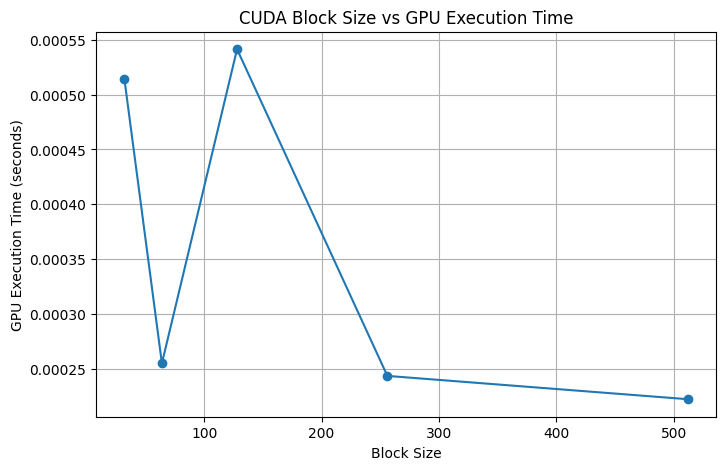
\includegraphics[width=0.7\textwidth]{bs.png}
\caption{CUDA block size vs GPU execution time.}
\label{fig}
\end{figure}

\end{document}
